Our approach to implementing explicit bypassing to fit it in our compiler within LLVM is to allocate the available bypasses sources during one of the compiler stages. The major compilation phases in LLVM are illustrated in Figure \ref{fig:phase_ordering}.  The first block represents instruction legalization, instruction lowering, and instruction selection, In general, we have that first the instructions are scheduled, then register allocation (RA) is performed, and finally, the instructions are printed in assembly language. Although one can use a post-RA scheduler to change the order in which to do scheduling and register allocation. At some point, we have to allocate our bypasses, which we can do only after we have backend specific instruction, i.e. after instruction selection. However, we could do this during any of compilation stages that follow, i.e. before scheduling and register allocation, during scheduling and register allocation and at the end of compilation. Moreover, scheduling and register allocation is already a phase problem on its own, as we have mentioned in Chapter \ref{sec:scheduling_and_ra}. Altogether, this leads to many possible approaches and we will discuss some of them below.

\begin{figure}[H]
\centering
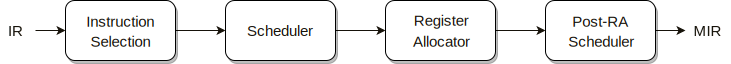
\includegraphics[width=.15\textwidth]{figures/phase_ordering}
\caption{Generalized code generation sequence.}
\label{fig:phase_ordering}
\end{figure}

\section{Last-minute Allocation}\label{sec:last_minute_alloc}
%Approach 1
One approach would be to allocate bypasses during the last stage of the compiler, just before printing the instructions. At this point, instructions are in order of execution and register allocation has already been performed and spill code has already been inserted in case we ran out of registers during RA. Because the order of instructions does not change at this point, the advantage of this approach is its simplicity. Namely, we could implement a pass that works on basic blocks, a basic block is a sequence of instructions with no branches, except for entering and leaving the basic block.

We could implement a pass to our backend that keeps track of the state of our pipeline in order to allocate our bypasses. Then we can determine for a cycle, which values currently reside in our bypass registers. Using this information we can then allocate bypasses and process the instructions in a top-down approach, demoting physical registers into bypass registers.

However, when we ran out of registers during register allocation, we had inserted spill code. When we allocate bypasses, we effectively free up registers. Since the spill code had already been inserted, it might have become unnecessary. Therefore, one improvement to this approach would be to move spill code after bypasses have been allocated to where they are needed, in order to avoid unnecessary spills.

\subsection{Advantages}
One of the advantages of this approach is its simplicity. Namely, the schedule is already given and variables have already been allocated to registers. Allocating bypasses with this information available is a relatively simpler problem. 

\subsection{Disadvantages}
Since the schedule is already given, there may be some additional bypassing opportunities that could have been used if the schedule would have been different. Therefore, some bypass opportunities may have been missed. Furthermore, this has currently been implemented as a pass that processes each basic block of a machine function. Desirable would be to extend the scope from basic block to a larger scope, e.g. extended basic blocks. 

\section{Bypass-aware Register Allocation}\label{sec:ra_approach}
%Approach 2
Another approach would be to implement a bypass-aware register allocator. Assuming that we have performed scheduling before register allocation, the instructions are in order of execution, allowing us to model the pipeline state as we did for the first approach. Our bypass-aware register allocator could start by allocating bypass registers. Then the remaining virtual registers could be allocated as usual. With this approach, we reduce register pressure by allocating bypasses before register allocation, effectively freeing registers. Therefore we may need less spill code, which is now inserted after bypasses have been allocated. So in contrary to the first approach, we do not have to take special care of spilling.

This approach would require us to implement a custom register allocator that consists of two phases. First, we allocate a bypass registers for each virtual register that can be bypassed. Subsequently, we have to allocate physical registers for the remaining virtual register. For the second phase, we may reuse any of the existing register allocators. 
%Introduce example code where we could have better bypass utilizzation, i.e. less stores by scheduling differently

\subsection{Advantages}
The main advantage of this approach is that it can deal efficiently with spill code. By effectively reducing register pressure before register allocation, we reduce the requirements on the register allocator.  
Since register allocation and bypass allocation are similar problems, it makes sense that these phases can be reordered. 

\subsection{Disadvantages}
Similar to last-minute allocation, the schedule is given prior to register allocation. Therefore, a schedule may exist that allows for better utilization of the bypass network. Therefore, we may gain in resulting code quality by controlling the resulting schedule.

\section{Bypass-aware Scheduling}\label{sec:scheduling_approach}
%Approach 3
For this approach, we need to implement a custom scheduler for our backend. This scheduler would prioritize to schedule instructions that may be bypassed close to each other, such that we may increase the possible number of bypasses. If we were to allocate bypasses during scheduling, some code may be inserted during register allocation or any other passes that follow, that may break a previously allocated bypass. Therefore, it may be wise to allocate the bypasses as late as possible, and let the scheduler be responsible for improving utilization of the bypass network. 

\subsection{Advantages}
By grouping instructions together such that they can be bypassed later on may increase the utilization of the bypass network and reduce accesses to the register file.

\subsection{Disadvantages}
Assuming that we have scheduled the code in such a way that we can efficiently use the bypass network, we still need to allocate the bypasses. We can use either one of the first two approaches to doing this and can, therefore, combine this approach with the first or second approach.

\section{Pre Scheduling Allocation}\label{sec:pre_scheduling}
%Approach 4
Before scheduling, we can identify instruction pairs that we can bypass. Then we change the virtual register that is bypassed into bypass registers and glue the two instructions together. This, however, makes restrictions on the resulting schedule. Since we group instruction together before scheduling, we may improve utilization of the bypass network. Namely, we may have grouped instruction together that otherwise would be scheduled far apart. This approach requires some new heuristics to determine whether it is profitable to group instruction together or when this may decrease efficiency, i.e. when grouping instructions decreases available ILP. 

When we allocate bypasses before scheduling and register allocation, it is possible that the scheduler or register allocator reorder instruction, or insert instruction, e.g. spill code, which breaks a previously allocated bypass. Therefore, a better approach would be to group instructions together as explained above but allocate the bypasses as late as possible, similar to the previous approach.

With this approach, we would need to find a tradeoff to not restrict the schedule too much, but still utilizing the bypass network as much as possible.   

\subsection{Advantages}
We may further increase utilization of the bypass network, reducing the total number of accesses to the register file. Furthermore, this approach may be combined with the previously proposed solutions. 

\subsection{Disadvantages}
As stated before, gluing nodes together introduces constraints on the schedule. We do not want to make too many restrictions on the schedule such that we decrease the efficiency of the compiled code. We do need to think of heuristics that may identify pairs of nodes which would increase the total number of bypasses if they were grouped together, and do that up to some point. Altogether, this means that it will be harder to develop because we should not do this too aggressively.

\section{Combined Scheduling and Register Allocation}\label{sec:combined_sched_ra}
%Approach 5 & 6
We can also choose to solve scheduling and RA in one go. This way, problems that can arise from doing one before the other may be avoided. There are two approaches to solve this problem. One is to solve it optimally, using constraint programming. Unison \cite{unison}, a separate project that solves scheduling and register allocation optimally in one go can be used with LLVM and can be extended to allocate our bypasses. However, solving this problem optimally may increase compilation time significantly, which we would like to avoid. Therefore, another approach would be to use heuristics to solve scheduling and register allocation in one go. There are no implementations of this thus far, which makes this approach the most difficult one. However, when we can efficiently deal with these problems in one go, we might extend this for other architectures as well. 

\subsection{Advantages}
Both approaches discussed in this section have the advantage that they do not have limitations that may be introduced by doing either scheduling or register allocation first. We, therefore, aim to increase the quality of the resulting code by merging the scheduling phase with the register allocation phase. 

\subsection{Disadvantages}
In general, combining register allocation and scheduling into one problem increases complexity, because these relatively difficult problems now need to be solved in one go. 
We have two variants of this approach, therefore we make a distinction between these two cases:
\begin{itemize}
\item Combined Scheduling and Register Allocation with Unison has as main disadvantage that compilation times increase since a constraint solver is usually time-consuming.
\item Combined Scheduling and Register Allocation with Heuristics only works as well as the heuristics that are used. Therefore, the main disadvantage of this approach is its implementation complexity. Choosing heuristics and developing the pass will require more work than the other approaches.
\end{itemize}